\documentclass[aspectratio=169]{beamer}
\usetheme{Boadilla}
\definecolor{MyUnivGreen}{RGB}{0,115,103}
\definecolor{MyUnivLight}{RGB}{229,242,240}
\definecolor{MyUnivRed}{RGB}{170,50,50}
\usecolortheme[named=MyUnivGreen]{structure}
\usefonttheme{serif}
\usepackage{cite}
\usepackage[table]{xcolor}
\usepackage{graphicx}
\usepackage{amsmath,amssymb,amsfonts}
\usepackage{booktabs}
\usepackage{tabularx}
\usepackage{array}
\usepackage{enumitem}
\usepackage{tikz}
\usetikzlibrary{arrows.meta,positioning,shapes.geometric}
\usepackage{ragged2e}
\logo{
\includegraphics[width=3.5cm,keepaspectratio]{images/logo/school_logo.png}}
\setbeamertemplate{navigation symbols}{}
\setbeamercolor{block title}{bg=MyUnivLight,fg=black}
\setbeamercolor{block body}{bg=white,fg=black}
\setbeamercolor{alertblock title}{bg=MyUnivRed!18,fg=MyUnivRed}
\setbeamercolor{alertblock body}{bg=MyUnivRed!5,fg=black}
\setlength{\tabcolsep}{3pt}
\renewcommand{\arraystretch}{1.15}
\setlist[itemize]{leftmargin=*,itemsep=1pt,topsep=2pt}
\setlist[enumerate]{leftmargin=*,itemsep=1pt,topsep=2pt}

\AtBeginSection[]{
    \begin{frame}{Outline}
        \tableofcontents[currentsection]
    \end{frame}}

\title[Capstone Project Introduction]{Review 1\\PROJ2999 Capstone Project Introduction}
\subtitle{\textbf{SYNAPSE-MAS: Shared Intelligent Memory Architecture for Multi-Agent LLM Systems}}
\author[Team No.]{Krishna Srinivas \and Aman Tej \and Sanjay Ramaswamy \and Ram Koushik\\[1mm]\small Guide: Dr. Srinivasa L. Chakravarthy}
\institute[GSCSE, GITAM]{Department of Artificial Intelligence and Data Science\\GITAM School of CSE\\GITAM Deemed to be University, Visakhapatnam}
\date{September 2026}
\titlegraphic{
\includegraphics[width=5cm]{images/logo/school_logo.png}}

\begin{document}
{\logo{}
\begin{frame}
\titlepage
\end{frame}}

\section{Introduction}
\begin{frame}{Multi-Agent Systems Need Memory}
\begin{columns}[T,onlytextwidth]
\begin{column}{0.48\textwidth}
\begin{block}{Why the problem matters}
\begin{itemize}
\item Specialized agents divide complex tasks and accumulate useful experience in parallel.
\item Conventional stateless agents lose that experience across sessions.
\item Repeated rediscovery wastes computation, tokens and time.
\end{itemize}
\end{block}
\end{column}
\begin{column}{0.48\textwidth}
\begin{alertblock}{Observed failure modes}
\begin{itemize}
\item Stale or contradictory memory may be reused.
\item Cross-agent knowledge transfer is weak and ad hoc.
\item Provenance, scope and consistency are difficult to govern.
\end{itemize}
\end{alertblock}
\end{column}
\end{columns}
\vspace{3mm}
\centering\large\textbf{The research need is a shared, selective and evolving memory layer.}
\end{frame}

\begin{frame}{Why Existing Approaches Fall Short}
\begin{columns}[T,onlytextwidth]
\begin{column}{0.31\textwidth}
\begin{block}{Stateless}
No persistent experience, no long-horizon continuity.
\end{block}
\end{column}
\begin{column}{0.31\textwidth}
\begin{block}{Retrieval-only / RAG}
Useful for access to stored context, but not inherently designed for memory admission, conflict resolution or evolution.
\end{block}
\end{column}
\begin{column}{0.31\textwidth}
\begin{block}{Static shared memory}
Shared state can become stale, noisy or contradictory without lifecycle control and governance.
\end{block}
\end{column}
\end{columns}
\vspace{3mm}
\begin{block}{The missing capability}
A memory architecture that can decide what to remember, what to reject, what to retrieve, and how to reconcile conflicting knowledge over time.
\end{block}
\end{frame}

\begin{frame}{Research Question}
\begin{alertblock}{Research Question}
\emph{``Can a selective, persistent and evolving shared-memory architecture improve the long-horizon performance, knowledge transfer and consistency of multi-agent LLM systems compared with conventional stateless and retrieval-only approaches?''}
\end{alertblock}
\end{frame}

\begin{frame}{SYNAPSE Architecture Concept}
\begin{center}
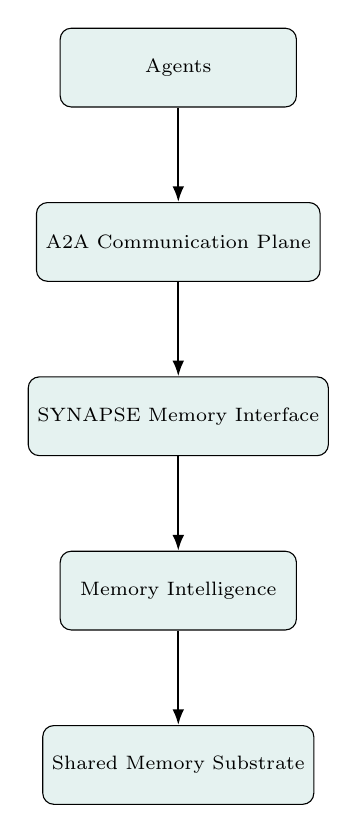
\begin{tikzpicture}[node distance=12mm, every node/.style={font=\scriptsize,align=center},
box/.style={draw,rounded corners,minimum height=10mm,minimum width=3.0cm,fill=MyUnivLight},
arrow/.style={-{Latex[length=2mm]},thick}]
\node[box] (agents) {Agents};
\node[box, below=of agents] (a2a) {A2A Communication Plane};
\node[box, below=of a2a] (iface) {SYNAPSE Memory Interface};
\node[box, below=of iface] (intel) {Memory Intelligence};
\node[box, below=of intel] (substrate) {Shared Memory Substrate};
\draw[arrow] (agents)--(a2a);
\draw[arrow] (a2a)--(iface);
\draw[arrow] (iface)--(intel);
\draw[arrow] (intel)--(substrate);
\end{tikzpicture}
\end{center}
\vspace{2mm}
\begin{block}{Key interpretation}
\textbf{A2A = talk now.}\quad\textbf{SYNAPSE = remember and reuse.}
Agents may communicate directly, while SYNAPSE selectively preserves reusable knowledge and governs evolution across sessions.
\end{block}
\end{frame}


\section{Literature Review}
\begin{frame}{Literature Review: Overview}
\begin{block}{Focus of the review}
This review examines how multi-agent LLM systems communicate, share knowledge and maintain useful memory across tasks and sessions.
\end{block}
\begin{columns}[T,onlytextwidth]
\begin{column}{0.48\textwidth}
\begin{block}{Themes across the literature}
\begin{itemize}
\item \textbf{Memory formation:} deciding what experience is worth retaining.
\item \textbf{Shared memory:} enabling agents to access common knowledge safely.
\item \textbf{Architecture:} organizing memory hierarchy, access and consistency.
\item \textbf{Governance:} controlling scope, provenance, ownership and updates.
\end{itemize}
\end{block}
\end{column}
\begin{column}{0.48\textwidth}
\begin{block}{Six-paper review path}
\begin{itemize}
\item Selective persistent memory
\item Governed shared memory
\item Computer-architecture perspective
\item Mesh memory protocol
\item Adaptive memory lifecycle
\item Change-intent and write governance
\end{itemize}
\end{block}
\end{column}
\end{columns}
\vspace{2mm}
\begin{alertblock}{Review direction}
The detailed review moves from communication and shared state to selective admission, provenance, conflict handling and long-term memory evolution. The final summary compares the papers and identifies the gap addressed by SYNAPSE-MAS.
\end{alertblock}
\end{frame}

\begin{frame}{Literature Review (Paper 1)}
\begin{columns}[T]
  \begin{column}{0.25\textwidth}
    \begin{block}{Title of the paper \cite{pedada26}}
      \tiny \textbf{Shared Selective Persistent Memory for Agentic LLM Systems}\\[2pt] Sanjana Pedada, Aditya Dhavala, Neelraj Patil (2026).\\[2pt] Problem: preserve reusable context across multi-turn agent sessions without retaining irrelevant reasoning history.
    \end{block}
    \vspace{0.12cm}
    \begin{block}{Main contributions}
      \tiny
      \begin{itemize}\setlength\itemsep{1pt}
      \item Selective retention of task specifications, data schemas, tool configurations and output constraints.
\item Shared persistent workspaces with role-based access.
\item Separates reusable context from session-specific reasoning traces.
\item Introduces zero-token data refresh for recurring updates.
      \end{itemize}
    \end{block}
    \vspace{0.12cm}
    \begin{block}{Inputs and Outputs}
      \tiny Agent interaction/task context and reusable workspace information are processed into persistent shared memory; the output is reusable contextual memory and refreshed artifacts.
    \end{block}
  \end{column}

  \begin{column}{0.4\textwidth}
    \begin{block}{Methodology}
    \tiny
    \begin{center}
    \textbf{Selective shared persistent memory}
    \end{center}
    \begin{itemize}\setlength\itemsep{1pt}
    \item Identify reusable context categories.
\item Discard session-specific traces and persist selected knowledge.
\item Reuse stored context across sessions/users.
\item Evaluate task completion and refresh efficiency.
    \end{itemize}
    \end{block}

    \begin{block}{Tools and Technology used}
      \tiny LLM-based agentic code-generation system; persistent memory/workspace; git-versioned artifacts; heterogeneous data sources; role-based access control.
    \end{block}
  \end{column}

  \begin{column}{0.25\textwidth}
    \begin{block}{Summary of Results}
      \tiny \textbf{96\%} task completion with memory vs. 79\% without memory and 71\% with full history in the reported enterprise scenarios. Zero-token refresh reduced task time by 14$\times$; summary-driven generation reduced token cost by 97$\times$.
    \end{block}
    \vspace{0.12cm}
    \begin{block}{Major Findings}
      \tiny
      \begin{itemize}\setlength\itemsep{1pt}
      \item Memory quality matters more than memory quantity.
\item Full-history persistence can degrade performance because of stale traces.
\item Selective memory supports collaborative reuse and efficiency.
      \end{itemize}
    \end{block}
  \end{column}
  \end{columns}
\end{frame}

\begin{frame}{Literature Review (Paper 2)}
\begin{columns}[T]
  \begin{column}{0.25\textwidth}
    \begin{block}{Title of the paper \cite{ref2}}
      \tiny \textbf{Governed Shared Memory for Multi-Agent LLM Systems}\\[2pt] Yanki Margalit, Nurit Cohen-Inger, Erni Avram, Ran Taig, Oded Margalit (2026).\\[2pt] Problem: shared multi-agent memory can suffer from unauthorized leakage, stale propagation, contradictions and loss of provenance.
    \end{block}
    \vspace{0.12cm}
    \begin{block}{Main contributions}
      \tiny
      \begin{itemize}\setlength\itemsep{1pt}
      \item Formalizes the fleet-memory problem.
\item Defines scoped retrieval and temporal supersession.
\item Adds provenance tracking and policy-governed propagation.
\item Evaluates governance through a reproducible harness.
      \end{itemize}
    \end{block}
    \vspace{0.12cm}
    \begin{block}{Inputs and Outputs}
      \tiny Agent/fleet memory is admitted and propagated under scope, temporal and provenance controls; outputs are governed shared memory with traceable derivations.
    \end{block}
  \end{column}

  \begin{column}{0.4\textwidth}
    \begin{block}{Methodology}
    \tiny
    \begin{center}
    \textbf{Governed shared-memory service + evaluation harness}
    \end{center}
    \begin{itemize}\setlength\itemsep{1pt}
    \item Define four governance failure modes.
\item Apply scope and propagation policies.
\item Track writer identity and derivation lineage.
\item Test governance behaviour under live service conditions.
    \end{itemize}
    \end{block}

    \begin{block}{Tools and Technology used}
      \tiny MemClaw multi-tenant memory service; ArgusFleet evaluation harness; scoped retrieval; provenance and policy controls.
    \end{block}
  \end{column}

  \begin{column}{0.25\textwidth}
    \begin{block}{Summary of Results}
      \tiny Reported 100\% reconstruction of depth-four provenance chains with correct writer identity and zero cross-fleet leakage under the tested conditions. The study also exposed scope-enforcement and pipeline-ordering issues.
    \end{block}
    \vspace{0.12cm}
    \begin{block}{Major Findings}
      \tiny
      \begin{itemize}\setlength\itemsep{1pt}
      \item Long-context retrieval alone is insufficient for governed shared memory.
\item Governance must be explicit at the systems level.
\item Pipeline ordering can affect contradiction handling.
      \end{itemize}
    \end{block}
  \end{column}
  \end{columns}
\end{frame}

\begin{frame}{Literature Review (Paper 3)}
\begin{columns}[T]
  \begin{column}{0.25\textwidth}
    \begin{block}{Title of the paper \cite{memoryarch26}}
      \tiny \textbf{Multi-Agent Memory from a Computer Architecture Perspective: Visions and Challenges Ahead}\\[2pt] Zhongming Yu, Naicheng Yu, Hejia Zhang, Wentao Ni, Mingrui Yin, Jiaying Yang, Yujie Zhao, Jishen Zhao (2026).\\[2pt] Problem: multi-agent memory is becoming a systems/architecture bottleneck involving hierarchy, access and consistency.
    \end{block}
    \vspace{0.12cm}
    \begin{block}{Main contributions}
      \tiny
      \begin{itemize}\setlength\itemsep{1pt}
      \item Frames multi-agent memory as a computer-architecture problem.
\item Distinguishes shared and distributed memory paradigms.
\item Proposes a three-layer I/O--cache--memory hierarchy.
\item Identifies cache-sharing and structured-access-control protocol gaps.
      \end{itemize}
    \end{block}
    \vspace{0.12cm}
    \begin{block}{Inputs and Outputs}
      \tiny Conceptual architectural analysis of multi-agent memory, mapping computer-architecture abstractions to agent memory and identifying open protocol/consistency problems.
    \end{block}
  \end{column}

  \begin{column}{0.4\textwidth}
    \begin{block}{Methodology}
    \tiny
    \begin{center}
    \textbf{Architectural / position framework}
    \end{center}
    \begin{itemize}\setlength\itemsep{1pt}
    \item Compare shared vs. distributed memory.
\item Map I/O, cache and memory layers to agent systems.
\item Examine access protocols and consistency requirements.
\item Identify open research directions.
    \end{itemize}
    \end{block}

    \begin{block}{Tools and Technology used}
      \tiny Computer-architecture abstractions; memory hierarchy; access protocols; consistency mechanisms. The paper is a position paper rather than an empirical model benchmark.
    \end{block}
  \end{column}

  \begin{column}{0.25\textwidth}
    \begin{block}{Summary of Results}
      \tiny The paper argues that \textbf{multi-agent memory consistency} is a central open challenge and that hierarchical memory plus explicit protocols are needed for reliable, scalable systems.
    \end{block}
    \vspace{0.12cm}
    \begin{block}{Major Findings}
      \tiny
      \begin{itemize}\setlength\itemsep{1pt}
      \item Memory should be treated as an architectural subsystem.
\item Consistency is not solved merely by providing shared storage.
\item Protocol design and structured access remain open problems.
      \end{itemize}
    \end{block}
  \end{column}
  \end{columns}
\end{frame}

\begin{frame}{Literature Review (Paper 4)}
\begin{columns}[T]
  \begin{column}{0.25\textwidth}
    \begin{block}{Title of the paper \cite{ref4}}
      \tiny \textbf{Mesh Memory Protocol: Semantic Infrastructure for Multi-Agent LLM Systems}\\[2pt] Hongwei Xu (2026).\\[2pt] Problem: agents collaborating across sessions need a semantic protocol for deciding what peer knowledge to accept, tracing its origin and preserving useful knowledge after restart.
    \end{block}
    \vspace{0.12cm}
    \begin{block}{Main contributions}
      \tiny
      \begin{itemize}\setlength\itemsep{1pt}
      \item Defines field-level rather than whole-message admission.
\item Provides inter-agent lineage for claims.
\item Stores the receiver's role-evaluated understanding rather than raw peer signals.
\item Specifies a semantic infrastructure layer for cross-session collaboration.
      \end{itemize}
    \end{block}
    \vspace{0.12cm}
    \begin{block}{Inputs and Outputs}
      \tiny Peer cognitive memory is evaluated field-by-field, linked to provenance/lineage, then transformed into receiver-side persistent memory for later reuse.
    \end{block}
  \end{column}

  \begin{column}{0.4\textwidth}
    \begin{block}{Methodology}
    \tiny
    \begin{center}
    \textbf{Mesh Memory Protocol (MMP)}
    \end{center}
    \begin{itemize}\setlength\itemsep{1pt}
    \item CAT7 represents Cognitive Memory Blocks.
\item SVAF evaluates fields against role-indexed anchors.
\item Content-hash parents/ancestors provide lineage.
\item Remix stores the receiver's evaluated understanding.
    \end{itemize}
    \end{block}

    \begin{block}{Tools and Technology used}
      \tiny Cognitive Memory Blocks (CMB); CAT7 schema; SVAF admission; content-hash lineage; receiver-side remix; agent identity and persistent memory.
    \end{block}
  \end{column}

  \begin{column}{0.25\textwidth}
    \begin{block}{Summary of Results}
      \tiny The paper reports three reference deployments in which autonomous agents collaborate across sessions using the specified semantic memory protocol.
    \end{block}
    \vspace{0.12cm}
    \begin{block}{Major Findings}
      \tiny
      \begin{itemize}\setlength\itemsep{1pt}
      \item Shared memory should not blindly copy peer messages.
\item Admission, provenance and receiver-side interpretation are distinct requirements.
\item This directly supports SYNAPSE's selective-admission and lineage design.
      \end{itemize}
    \end{block}
  \end{column}
  \end{columns}
\end{frame}

\begin{frame}{Literature Review (Paper 5)}
\begin{columns}[T]
  \begin{column}{0.25\textwidth}
    \begin{block}{Title of the paper \cite{ama26}}
      \tiny \textbf{AMA: Adaptive Memory via Multi-Agent Collaboration}\\[2pt] arXiv:2601.20352 (2026).\\[2pt] Problem: multi-agent systems need memory that can adapt to task context and uncertainty instead of relying on a fixed memory schema.
    \end{block}
    \vspace{0.12cm}
    \begin{block}{Main contributions}
      \tiny
      \begin{itemize}\setlength\itemsep{1pt}
      \item Introduces explicit memory lifecycle stages across formation and update.
\item Uses varying retrieval granularity and query routing.
\item Incorporates judgement, retry and conflict detection.
\item Supports refresh and targeted memory update when evidence is insufficient.
      \end{itemize}
    \end{block}
    \vspace{0.12cm}
    \begin{block}{Inputs and Outputs}
      \tiny Agent experience, task queries and evidence are transformed into adaptive memory updates and context-specific retrieval decisions.
    \end{block}
  \end{column}

  \begin{column}{0.4\textwidth}
    \begin{block}{Methodology}
    \tiny
    \begin{center}
    \textbf{Adaptive memory lifecycle}
    \end{center}
    \begin{itemize}\setlength\itemsep{1pt}
    \item Extract reusable experience from agent actions.
\item Route retrieval based on task query and memory granularity.
\item Judge reliability and sufficiency of evidence.
\item Refresh or revise memory when conflicts or gaps emerge.
    \end{itemize}
    \end{block}

    \begin{block}{Tools and Technology used}
      \tiny Multi-agent collaboration patterns; adaptive retrieval; lifecycle-based memory control; evidence-aware update logic.
    \end{block}
  \end{column}

  \begin{column}{0.25\textwidth}
    \begin{block}{Summary of Results}
      \tiny The paper highlights adaptive memory as a dynamic lifecycle, where agents decide when to retrieve, when to retry and when to revise memory based on evidence quality.
    \end{block}
    \vspace{0.12cm}
    \begin{block}{Major Findings}
      \tiny
      \begin{itemize}\setlength\itemsep{1pt}
      \item Memory must adapt to task context and uncertainty.
\item Retrieval should not be fixed at one granularity.
\item Judgement and refresh are necessary for durable memory quality.
      \end{itemize}
    \end{block}
    \begin{alertblock}{SYNAPSE Adapts}
      \tiny SYNAPSE adopts the lifecycle idea as formation $\rightarrow$ selective admission $\rightarrow$ judgement $\rightarrow$ conflict resolution $\rightarrow$ consolidation $\rightarrow$ evolution.
    \end{alertblock}
  \end{column}
  \end{columns}
\end{frame}

\begin{frame}{Literature Review (Paper 6)}
\begin{columns}[T]
  \begin{column}{0.25\textwidth}
    \begin{block}{Title of the paper \cite{claimplane26}}
      \tiny \textbf{Claim Plane: Enforceable Change Intents and Dynamic Scope}\\[2pt] arXiv:2607.21909 (2026).\\[2pt] Problem: concurrent agents need a disciplined mechanism for deciding whether a write or change should be admitted under ambiguity or conflict.
    \end{block}
    \vspace{0.12cm}
    \begin{block}{Main contributions}
      \tiny
      \begin{itemize}\setlength\itemsep{1pt}
      \item Defines pre-write admission and intent tracking.
\item Emphasizes fail-closed behavior under ambiguity.
\item Supports change scope and version-aware enforcement.
\item Links provenance to write control decisions.
      \end{itemize}
    \end{block}
    \vspace{0.12cm}
    \begin{block}{Inputs and Outputs}
      \tiny Proposed change intents, scope constraints and provenance signals are evaluated before a write is accepted; the output is an enforceable update or rejection decision.
    \end{block}
  \end{column}

  \begin{column}{0.4\textwidth}
    \begin{block}{Methodology}
    \tiny
    \begin{center}
    \textbf{Deterministic write admission}
    \end{center}
    \begin{itemize}\setlength\itemsep{1pt}
    \item Define the intended change before write execution.
\item Validate scope and version constraints.
\item Refuse ambiguous or unsafe updates.
\item Preserve lineage and provenance metadata.
    \end{itemize}
    \end{block}

    \begin{block}{Tools and Technology used}
      \tiny Deterministic scope enforcement, change-intent governance, version tracking, provenance-aware update control, fail-closed decision logic.
    \end{block}
  \end{column}

  \begin{column}{0.25\textwidth}
    \begin{block}{Summary of Results}
      \tiny The paper presents a strong engineering principle: when intent is uncertain, the correct system behavior is conservative rejection rather than unsafe propagation.
    \end{block}
    \vspace{0.12cm}
    \begin{block}{Major Findings}
      \tiny
      \begin{itemize}\setlength\itemsep{1pt}
      \item Intent-aware admission is critical in concurrent settings.
\item Provenance and versioning are not optional extras.
\item Fail-closed behavior improves reliability under ambiguity.
      \end{itemize}
    \end{block}
    \begin{alertblock}{SYNAPSE Adapts}
      \tiny SYNAPSE uses the same principle for memory-write governance, conflict admission, lineage tracking and controlled memory evolution.
    \end{alertblock}
  \end{column}
  \end{columns}
\end{frame}


\section{Summary of Literature Review}
\begin{frame}{Summary of Literature Review}
\scriptsize
\begin{tabularx}{\textwidth}{p{0.14\textwidth}p{0.25\textwidth}p{0.18\textwidth}p{0.18\textwidth}X}
\toprule
\textbf{Ref.} & \textbf{Overview of Paper} & \textbf{Model / Approach} & \textbf{Novelty / Contribution} & \textbf{Limitations / Scope} \\
\midrule
\cite{pedada26} & Selective persistent memory & structured memory + admission & reusable task specifications and memory quality & enterprise/workspace context; no shared multi-agent governance\\
\cite{margalit26} & Governed shared memory & provenance + temporal validity + scope control & policy-governed shared state & governance-centric, not full lifecycle intelligence\\
\cite{memoryarch26} & Architecture framing & memory hierarchy and consistency view & shared vs distributed memory analysis & conceptual/position framing\\
\cite{xu26} & Mesh memory protocol & receiver-side semantic admission + lineage & semantic infrastructure for exchange & protocol-level scope, not full memory intelligence\\
\cite{ama26} & Adaptive memory & lifecycle roles + targeted refresh & judgement, conflict, granularity & different architecture/context\\
\cite{claimplane26} & Change-intent governance & deterministic write admission + scope enforcement & provenance + fail-closed control & coding-agent setting; not a general memory architecture\\
\bottomrule
\end{tabularx}
\vspace{2mm}
\begin{block}{Overall Observation}
The six core papers collectively establish the need for selective admission, provenance, governance, conflict handling and memory evolution. SYNAPSE integrates these concerns into a shared, persistent and evolving multi-agent memory layer.
\end{block}
\end{frame}


\section{Research Gaps}
\begin{frame}{Research Gaps}
\begin{block}{Observations from Literature}
The literature shows value in selective memory, provenance, retrieval relevance, and layered multi-agent architecture, but these ideas are typically addressed in isolation rather than as one integrated memory lifecycle.
\end{block}
\begin{alertblock}{Identified Gaps}
\begin{itemize}[leftmargin=1.5em,itemsep=4pt,topsep=4pt]
\item \textbf{Selective admission and memory quality.} Existing work demonstrates the value of selective memory, but SYNAPSE studies this in a shared multi-agent setting with additional judgement and lifecycle control.
\item \textbf{Governed shared memory.} Prior work addresses provenance, scope and temporal validity, but SYNAPSE integrates governance across formation, retrieval, update and evolution.
\item \textbf{Semantic conflict resolution.} Storage consistency alone does not guarantee semantic consistency; SYNAPSE treats judgement and conflict resolution as memory-intelligence operations.
\item \textbf{Long-horizon memory evolution.} A lifecycle beyond store $\rightarrow$ retrieve is needed; SYNAPSE investigates form $\rightarrow$ admit $\rightarrow$ retrieve $\rightarrow$ judge $\rightarrow$ resolve $\rightarrow$ consolidate $\rightarrow$ evolve.
\item \textbf{Cross-agent knowledge transfer.} A2A enables communication, but communication does not automatically create reusable persistent knowledge; SYNAPSE separates the communication plane from the memory plane.
\end{itemize}
\end{alertblock}
\end{frame}


\section{Problem Statement}
\begin{frame}{Problem Statement}
\begin{exampleblock}{Problem Statement}
To design and evaluate a shared intelligent memory architecture for multi-agent LLM systems that enables agents to selectively store, retrieve, share, consolidate and evolve knowledge and experiences across interactions, while maintaining relevance, consistency, provenance and efficient memory usage.
\end{exampleblock}
\vspace{4mm}
\begin{block}{Research Direction}
SYNAPSE-MAS studies a shared memory architecture in which memory is a governed coordination substrate rather than a passive vector store or an implicit conversation transcript.
\end{block}
\end{frame}


\section{Research Objectives}
\begin{frame}{Project Objectives}
\begin{exampleblock}{Objectives}
\begin{itemize}[leftmargin=1.5em,itemsep=4pt,topsep=4pt]
\item Design and implement a shared memory architecture supporting persistent episodic and semantic memory with contextual retrieval.
\item Develop selective memory formation and evolution mechanisms for relevance-based admission, redundancy reduction, conflict resolution, consolidation and updating/evolution.
\item Evaluate SYNAPSE-MAS against the stateless baseline, the retrieval-only / RAG baseline and the static/shared-memory baseline using task performance, retrieval quality, memory efficiency, cross-agent knowledge transfer and consistency.
\end{itemize}
\end{exampleblock}
\vspace{3mm}
\begin{block}{Evaluation metrics}
Measured outcomes include task performance, retrieval quality, memory efficiency, cross-agent knowledge transfer, consistency, token usage, latency and storage growth.
\end{block}
\end{frame}

\begin{frame}{Proposed System Direction -- SYNAPSE-MAS}
\centering
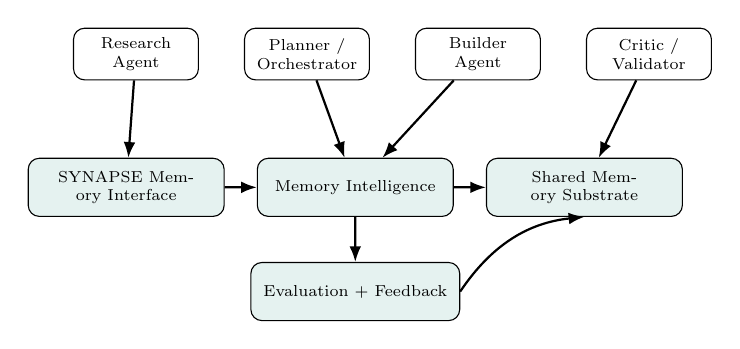
\begin{tikzpicture}[scale=.82,transform shape,node distance=6mm and 7mm, every node/.style={font=\scriptsize,align=center},
box/.style={draw,rounded corners,minimum height=9mm,text width=2.8cm,fill=MyUnivLight},
agent/.style={draw,rounded corners,minimum height=8mm,text width=1.7cm,fill=white},
arrow/.style={-{Latex[length=2mm]},thick}]
\node[agent] (planner) {Planner /\\Orchestrator};
\node[agent,left=of planner] (research) {Research\\Agent};
\node[agent,right=of planner] (builder) {Builder\\Agent};
\node[agent,right=of builder] (critic) {Critic /\\Validator};
\node[box,below=12mm of planner,xshift=-2.8cm] (interface) {SYNAPSE Memory Interface};
\node[box,right=5mm of interface] (intel) {Memory Intelligence};
\node[box,right=5mm of intel] (store) {Shared Memory Substrate};
\node[box,below=7mm of intel,text width=3.0cm] (eval) {Evaluation + Feedback};
\draw[arrow] (research)--(interface);
\draw[arrow] (planner)--(intel);
\draw[arrow] (builder)--(intel);
\draw[arrow] (critic)--(store);
\draw[arrow] (interface)--(intel);
\draw[arrow] (intel)--(store);
\draw[arrow] (intel)--(eval);
\draw[arrow] (eval.east) to[bend left=25] (store.south);
\end{tikzpicture}
\vspace{1mm}
\small\textbf{Key idea:} A2A supports communication, while SYNAPSE governs the durable memory plane for retrieval, validation, conflict handling and memory evolution.
\end{frame}


\section{Workplan and Proposed Timeline}
\begin{frame}{Work Breakdown and Task Allocation}
\scriptsize
\begin{tabularx}{\textwidth}{p{0.24\textwidth}p{0.20\textwidth}X}
\toprule
\textbf{Task Area} & \textbf{Primary Owner} & \textbf{Key Responsibilities} \\
\midrule
Problem framing and literature synthesis & Krishna & Identify research question, review core papers, derive gaps and structure the Review-I presentation \\
Architecture and agent interfaces & Sanjay & Define agent layers, A2A communication, memory interface and orchestration boundaries \\
Storage, indexing and retrieval & Ram & Persistent storage design, structured and vector memory, retrieval APIs, metadata handling \\
Memory intelligence and testing & Aman & Selective admission, conflict handling, consolidation, evaluation design and ablation tests \\
End-to-end integration and analysis & All & Prototype integration, validation, reporting and Review-II preparation \\
\bottomrule
\end{tabularx}
\end{frame}

\begin{frame}{Proposed Timeline and Milestones}
\scriptsize
\begin{tabularx}{\textwidth}{p{0.24\textwidth}p{0.20\textwidth}p{0.16\textwidth}p{0.18\textwidth}p{0.18\textwidth}}
\toprule
\textbf{Milestone} & \textbf{Status} & \textbf{Window} & \textbf{Owner} & \textbf{Focus} \\
\midrule
M1: Problem formulation and literature review & \textbf{Completed} & Sep 2026 & Krishna & Research question, problem statement, literature synthesis \\
M2: Architecture and requirements baseline & \textbf{In Progress} & Oct 2026 & Sanjay + Ram & Memory interface, component boundaries, governance requirements \\
M3: Shared-memory prototype & \textbf{Planned} & Oct-Nov 2026 & Ram + Sanjay & Storage, retrieval, metadata, provenance \\
M4: Memory intelligence and conflict mechanisms & \textbf{Planned} & Nov 2026 & Aman & Admission, judgement, consolidation, evolution \\
M5: Baselines and experimental evaluation & \textbf{Planned} & Nov-Dec 2026 & All & Task performance, memory efficiency, transfer and consistency \\
M6: Review-II preparation & \textbf{Planned} & Dec 2026 & All & Analysis, reporting and presentation refinement \\
\bottomrule
\end{tabularx}
\vspace{3mm}
\begin{block}{Timeline interpretation}
The architecture and prototype tasks are currently in progress or planned, while the Review-I research framing and the literature synthesis are the completed foundation for the project.
\end{block}
\end{frame}


\section{Action Plan}
\begin{frame}{Action Plan}
\begin{itemize}[leftmargin=1.5em,itemsep=4pt,topsep=4pt]
\item Freeze the architecture boundary between A2A communication and SYNAPSE memory operations.
\item Implement the memory interface with storage, retrieval and provenance metadata.
\item Implement persistent episodic and semantic memory with contextual retrieval using a minimal prototype pipeline.
\item Add memory-intelligence services for selective admission, redundancy reduction, judgement and conflict resolution.
\item Implement consolidation and evolution routines that update memory lineage and maintain semantic consistency.
\item Compare SYNAPSE-MAS against stateless, retrieval-only and static shared-memory baselines.
\item Analyze task performance, retrieval quality, memory efficiency, transfer and consistency to prepare Review-II.
\end{itemize}
\vspace{2mm}
\begin{exampleblock}{Immediate next milestone}
A working prototype that demonstrates traceable memory formation, selective retrieval and cross-agent knowledge reuse within the SYNAPSE layer.
\end{exampleblock}
\end{frame}


\section*{References}
\begin{frame}[allowframebreaks]{References}
\scriptsize
\bibliographystyle{unsrt}
\bibliography{ref}
\end{frame}

\section{Disclosure Statements}
\begin{frame}{Disclosure Statements}
\begin{itemize}
\item I will maintain academic honesty by doing my own work and avoiding plagiarism, cheating, unauthorized collaboration, falsifying information, and misuse of AI-generated content.
\item I will properly acknowledge and cite all sources used, including papers, websites, software and AI tools.
\item I will use institutional resources responsibly and only for authorized academic or research activities.
\item I understand that I remain responsible for the correctness, originality and decisions in the submitted work.
\end{itemize}
\end{frame}


\end{document}
